\documentclass[12pt]{extarticle}
%%%%%%%%%%%%%%% PACKAGES %%%%%%%%%%%%%%%
\usepackage{titleps}
\usepackage{url}
\usepackage{amsmath}
\usepackage{cancel}
\usepackage{amsfonts}
\usepackage{amssymb}
\usepackage{mathtools}
\usepackage{graphicx}
\usepackage[dvipsnames]{xcolor}
\usepackage[colorlinks]{hyperref}
\usepackage{geometry}
\geometry{
    a4paper,
    left=19mm,
    right=19mm,
    top=20mm,
    bottom=25mm
}
% Define dark and mid color

\definecolor{Sepia}{HTML}{704214}
\definecolor{RedViolet}{HTML}{C71585}

% Mix lighter shade

\colorlet{LightSepia1}{Sepia!80!yellow}
\colorlet{LightSepia2}{Sepia!70!orange}
\colorlet{DarkGolden}{RedViolet!30!yellow!70!Maroon!70!Brown}
\colorlet{Golden}{RedViolet!30!yellow!70!pink!90!Brown}
\colorlet{DDarkGolden}{RedViolet!20!yellow!70!Maroon!70!Black!65!Brown}

%%%%%%%%%%%%%%%%%%%%%%%%%%%%%%%%%%%%%%%%
%%%%%%%%%%%%%%% FONT %%%%%%%%%%%%%%%%%%%
\usepackage[T1]{fontenc}
\usepackage{charter}

\def\primarycolor{DarkGolden}
\def\secondarycolor{Golden}
%%%%%%%%%%%%%%%%%%%%%%%%%%%%%%%%%%%%%%%%
%%%%%%%%%%%%%%% HEADER %%%%%%%%%%%%%%%%%
\usepackage{fancyhdr}
\let\oldheadrule\headrule
\renewcommand{\headrule}{\color{\secondarycolor}\oldheadrule}
\renewcommand{\headrulewidth}{0.7pt}
\pagestyle{fancy}
\fancyhead{}\fancyfoot{}
\fancyhead[L]{\scshape \large \color{\primarycolor}{\fontfamily{qpl}\selectfont
Amirreza "Farnam" Taheri \\
Student ID: 4021300198003
}}
\fancyhead[R]{\color{\secondarycolor} Game Theory}
\fancyfoot[C]{\textcolor{\primarycolor}{(\thepage)}}
\setlength{\headheight}{1cm}

\fancypagestyle{headerpage}{
    \fancyhf{} % Clear header and footer
    \renewcommand{\headrulewidth}{0pt} % Remove header rule
    \renewcommand{\footrulewidth}{0pt} % Remove footer rule
    \fancyhead[R]{} % Remove the line that displays "Course Name (Course Code)" in the header page
}

%%%%%%%%%%%%%%%%%%%%%%%%%%%%%%%%%%%%%%%%
%%%%%%%%%%%%%%% COMMANDS %%%%%%%%%%%%%%%
% \newcommand{\norm}[1]{\lVert#1\rVert}
% \newcommand{\inner}[1]{\langle#1\rangle}
\newcommand{\problem}[1]{
    \subsection*{\textcolor{\secondarycolor}{#1}}
    \addcontentsline{toc}{subsection}{\protect\numberline{}#1}
}
\newcommand{\partof}[1]{
    \subsubsection*{\textcolor{\secondarycolor}{(#1)}}
    \addcontentsline{toc}{subsubsection}{\protect\numberline{}#1}
}
%%%%%%%%%%%%%%%%%%%%%%%%%%%%%%%%%%%%%%%%
%%%%%%%%%%%%%%% BODY %%%%%%%%%%%%%%%%%%%
\linespread{1.4}
\color{DDarkGolden}
\begin{document}
\setlength{\abovedisplayskip}{6pt}
\setlength{\belowdisplayskip}{6pt}
\setlength{\abovedisplayshortskip}{0pt}
\setlength{\belowdisplayshortskip}{0pt}
%%%%%%%%%%%%%%% CONTENT %%%%%%%%%%%%%%%%
\thispagestyle{headerpage} % Apply custom header style to this page only
\begin{center}
    \vspace*{1.5cm}
    {\Huge\bfseries\color{\primarycolor}{\fontfamily{qpl}\selectfont Exercise 3}} \\
    \vspace{3cm}
    
\includegraphics[width=6cm]{teias.png} \\ % Replace "university_logo.png" with the actual filename of your university logo
    \vspace{2cm}
    {\Large\color{\primarycolor}{\fontfamily{qpl}\selectfont Amirreza "Farnam" Taheri}} \\
    {\large\color{\primarycolor}{Student ID: 4021300198003}} \\
    \vspace{3cm}
    {\large\bfseries\color{\secondarycolor}{Macroeconomics I}} \\
    \vspace{1cm}
    {\large\color{\secondarycolor}{Instructor: Prof. Hosein Joshaghani}} \\
    \vspace{3cm}
    {\large\color{\secondarycolor}{March 11, 2024}} % Replace with the actual date or semester information
\end{center}
\newpage % Add a page break after the header page

%%%%%%%%%%%%%%% CONTENT %%%%%%%%%%%%%%%%
\pagestyle{fancy} % Apply fancy header to the remaining pages
\fancyhead[R]{\color{\secondarycolor} Problemset 3} % Display "Problemset #no" in the header of the remaining pages
%%%%%%%%%%%%%%%%%%%%%%%%%%%%%%%%%%%%%%%%
%%%%%%%%%%%%%%%%%%%%%%%%%%%%%%%%%%%%%%%%
\textbf{\Large\begin{center}
    {Neoclassical Growth Model}
\end{center}}
\textbf{\large\begin{center}
    {Centralized Economy in Discrete Time}
\end{center}}
Consider a discrete time model, where a central planner allocates output between consumption and investment.
$$y_t=c_t+i_t$$
Notice that the national income identity also serves as the resource constraint for the whole economy. Here
total output is also total income and this is either spent on consumption or is saved, $s_t = i_t$. As before, the
increase in the stock of capital (net investment) during period t equals new (gross) investment less depreciated
capital,
$$\Delta k_{t+1}=i_t-\delta k_t$$
An increase in the stock of capital increases output yt = F (kt), but at a diminishing rate, i.e., $F'(.) >
0,\;F''(.) < 0$. Also assume that the marginal product of capital approaches zero as capital tends to infinity and
that it approaches infinity as capital tends to zero (Inada conditions hold). Given an initial stock of capital kt
(the endowment), the economy must choose its preferred level of consumption for period $t\;:\;c_t$, and capital at
the start of period $t + 1 : k_{t+1}$. Assume that the economy values consumption today more than consumption
in the future, and wishes to solve the following problem:
$$\max_{c_{t+s},\;k_{t+s+1}}\sum_{s=0}^{\infty}\beta^s U(c_{t+s})$$
where $U'_t>0,\;U''_t<0$. Put $\beta=\dfrac{1}{1+\theta}$ such that $\theta>0$ and $0 < \beta < 1$.
\newpage
%%%%%%%%%%%%%%%%%%%%%%%%%%%%%%%%%%%%%%%%
%%%%%%%%%%%%%%%%%%%%%%%%%%%%%%%%%%%%%%%%
\problem{1.}Output and investment can be eliminated from the analysis and the model can be reduced to just one
equation involving two variables. By doing so, derive the resource constraint the economy faces as an
equation involving capital and consumption.\\\\\\
From the national income identity and the law of motion for capital, we have:
\begin{equation}
    y_t = c_t + i_t
\end{equation}
\begin{equation}
    \Delta k_{t+1} = i_t - \delta k_t 
\end{equation}\\
Substituting \( i_t \) from the equation $(2)$ into the equation $(1)$ gives us:
$$ y_t = c_t + \Delta k_{t+1} + \delta k_t $$\\
Since \( y_t = F(k_t) \), the resource constraint can be written as:
$$ F(k_t) = c_t + \Delta k_{t+1} + \delta k_t $$\\
This equation represents the resource constraint the economy faces, envolving consumption and capital across periods.
It shows that the total output produced by the capital stock must be allocated between consumption, new capital, and replacing the depreciated capital.%%%%%%%%%%%%%%%%%%%%%%%%%%%%%%%%%%%%%%%%
\newpage
%%%%%%%%%%%%%%%%%%%%%%%%%%%%%%%%%%%%%%%%
%%%%%%%%%%%%%%%%%%%%%%%%%%%%%%%%%%%%%%%%
\problem{2.}Find the Golden Rule, i.e., where the consumption is maximized subject to the additional constraint
that the level of consumption should be sustainable.\\\\\\
The steady-state condition is:
$$\Delta k_{t+1} = 0 = i_t - \delta k_t$$\\
Substituting $i_t = \delta k_t$ into the resource constraint,
we get:
$$F(k_t) = c_t + \delta k_t\; \implies \; c_t=F(k_t)-\delta k_t  $$\\
This equation represents theconsumption as a function of capital.
To find the Golden Rule level of capital, we need to maximize this function.\\\\
The first order condition is:
$$F'(k_t) - \delta = 0$$\\
So the Golden Rule would be:
$$F'(k_t) = \delta$$
\newpage
%%%%%%%%%%%%%%%%%%%%%%%%%%%%%%%%%%%%%%%%
%%%%%%%%%%%%%%%%%%%%%%%%%%%%%%%%%%%%%%%%
\problem{3.}Now, using the constraint in part $(1)$, write the Lagrangian for the maximization problem and derive
the first order conditions.\\\\\\
The Lagrangian for this problem is:\\
\begin{align*}
    \mathcal{L} &=\; \sum_{s=0}^{\infty}\beta^s[U(c_{t+s}) + \lambda_{t+s}(F(k_{t+s}) - c_{t+s} - \Delta k_{t+s+1} - \delta k_{t+s})]\\
    &=\;\sum_{s=0}^{\infty}\beta^s[U(c_{t+s}) + \lambda_{t+s}(F(k_{t+s}) - c_{t+s} - k_{t+s+1}+k_{t+s} - \delta k_{t+s})]
\end{align*}\\\\
The first order conditions are:\\
\setcounter{equation}{0}
\begin{align}
    \frac{\partial \mathcal{L}}{\partial c_{t+s}} =&\; 0 \Rightarrow U'(c_ {t+s}) - \lambda_{t+s} = 0\\
    \frac{\partial \mathcal{L}}{\partial k_{t+s+1}} =&\; 0 \Rightarrow \beta^{t+s}\lambda_{t+s} - \beta^{t+s+1}\lambda_{t+s+1}(F'(k_{t+s+1}) + (1-\delta)) = 0\\
    \frac{\partial \mathcal{L}}{\partial \lambda_{t+s}} =&\; 0 \Rightarrow F(k_{t+s}) - c_{t+s} - \Delta k_{t+s+1} - \delta k_{t+s} = 0
\end{align}
\newpage
%%%%%%%%%%%%%%%%%%%%%%%%%%%%%%%%%%%%%%%%
%%%%%%%%%%%%%%%%%%%%%%%%%%%%%%%%%%%%%%%%
\problem{4.}Using the first order conditions in part $(3)$, derive the Euler equation.\\\\\\
From the first order conditions, we have:
\setcounter{equation}{0}
\begin{align}
    &U'(c_{t+s}) - \lambda_{t+s} &= 0 \qquad\qquad\qquad\\
    &\beta^{t+s}\lambda_{t+s} - \beta^{t+s+1}\lambda_{t+s+1}(F'(k_{t+s+1}) + (1-\delta)) &= 0 \qquad\qquad\qquad\\
    &F(k_{t+s}) - c_{t+s} - \Delta k_{t+s+1} - \delta k_{t+s} &= 0 \qquad\qquad\qquad
\end{align}\\
From equation $(1)$, we can have:
$$\lambda_{t+s} = U'(c_{t+s})$$\\
Substituting $\lambda_{t+s}$ and $\lambda_{t+s+1}$ from equation $(1)$ into equation $(2)$, we get:\\
$$\beta^{t+s}U'(c_{t+s}) - \beta^{t+s+1}U'(c_{t+s+1})(F'(k_{t+s+1}) + (1-\delta)) = 0$$
$$\implies \frac{U'(c_{t+s})}{U'(c_{t+s+1})} = \beta (F'(k_{t+s+1}) + (1-\delta))$$\\
\newpage
%%%%%%%%%%%%%%%%%%%%%%%%%%%%%%%%%%%%%%%%
%%%%%%%%%%%%%%%%%%%%%%%%%%%%%%%%%%%%%%%%
\problem{5.} Using the resource constraint and the Euler equation, depict the phase diagram of c versus k.\\\\\\
The dynamic of capital is already given in the question:
$$\Delta k_{t+1}=i_t-\delta k_t$$\\\\
Now in order to draw the phase diagram, we must find dynamic of consumption.\\
From the previous part, we had Euler equation as:
$$ \frac{u'(c_t)}{u'(c_{t+1})} = \beta (F'(k_{t+1}) + 1 - \delta) $$\\
In order to Implementng the CRRA function by the following form into the Euler equation.\\\\
Utility function:
$$ U(c) = \frac{c^{1-1/\rho}}{1-1/\rho},\quad \rho > 0 $$\\
First derivative is:
$$U'(c) = c^{-1/\rho}$$\\
Second derivative is:
$$ U''(c) = -\frac{1}{\rho} c^{-1/\rho-1}$$\\
Substituting the derivatives of the utility function into the Euler equation, we have:
$$ \frac{c_{t+s}^{-1/\rho}}{c_{t+s+1}^{-1/\rho}} = \beta (F'(k_{t+s+1}) + (1-\delta)) $$\\
Simplifying, we get:
$$ \left(\frac{c_{t+s}}{c_{t+s+1}}\right)^{1/\rho} = \beta (F'(k_{t+s+1}) + 1-\delta)$$\\
Which can be further simplified as:
$$\frac{c_{t+s}}{c_{t+s+1}} = (\beta (F'(k_{t+s+1}) + (1-\delta)))^\rho$$
Now, in order to find the dynamic of consumption, let's log-linearize the equation:\\
\begin{align*}
    \ln\left(\frac{c_{t+s}}{c_{t+s+1}}\right) &= \rho \ln\left(\beta (F'(k_{t+s+1}) + 1-\delta)\right)\\
    \ln(c_{t+s}) - \ln(c_{t+s+1}) &= \rho \ln\left(\beta (F'(k_{t+s+1}) + 1-\delta)\right)\\
    \Delta c &\approx -\rho \ln\left(\beta (F'(k_{t+s+1}) + 1-\delta)\right)\\
\end{align*}
%%%%%%%%%%%%%%%%%%%%%%%%%%%%%%%%%%%%%%%%
So the dynamics of the system are:
\setcounter{equation}{0}
\begin{align}
    \Delta k &=i_t-\delta k_t\\
    \Delta c &= -\rho \ln\left(\beta (F'(k_{t+s+1}) + 1-\delta)\right)
\end{align}\\
Setting them equal to zero, we will get the steady states conditions:\\
\setcounter{equation}{0}
\begin{align}
    k_t&=\dfrac{i_t}{\delta}\\\notag\\
    \beta (F'(k_{t+s+1}) + (1-\delta))&=1\notag\\ 
    \implies F'(k_{t+s+1}) & = \dfrac{1}{\beta}+\delta-1 
\end{align}\\\\
Implementing a Cobb-Douglas production function in the form of $y_t=f(k_t)=k_t^\alpha$, we get:
\begin{align*}
    k^*=\left[(\dfrac{1}{\beta}+\delta-1)/\alpha\right]^{\frac{1}{\alpha-1}} \tag{2}
\end{align*}\\
Substitute \(k^*\) and \(y^*\) into the resource constraint to get the steady state level of consumption:

$$c^* = y^* - \delta k^* = \left[\frac{\frac{1}{\beta} + \delta - 1}{\alpha}\right]^\frac{\alpha}{\alpha-1} - \delta \left[\frac{\frac{1}{\beta} + \delta - 1}{\alpha}\right]^{1/(\alpha - 1)}$$

\newpage
%%%%%%%%%%%%%%%%%%%%%%%%%%%%%%%%%%%%%%%%
%%%%%%%%%%%%%%%%%%%%%%%%%%%%%%%%%%%%%%%%
%%%%%%%%%%%%%%%%%%%%%%%%%%%%%%%%%%%%%%%%
\textbf{\large\begin{center}
    {Numerical Analysis of the Neoclassical Growth Model}
\end{center}}
\vspace*{0.5cm}
In this question we want to simulate a neoclassical growth model and analyze how its structural parameters
change the dynamics of the model. Consider the problem that we studied in class.\\\\
\textbf{Model}\\
The representative household maximizes its lifetime utility
\begin{equation}
U = B \int_{t=0}^{\infty} e^{-\beta t} \dfrac{c(t)^{1-\theta}}{1-\theta} dt \tag{1}
\end{equation}\\
subject to its budget constraint
\begin{equation}
\int_{t=0}^{\infty} e^{-R(t)}c(t)e^{(n+g)t} dt \leq k(0) + \int_{t=0}^{\infty} e^{-R(t)}w(t)e^{(n+g)t} dt \tag{2}
\end{equation}\\
we also can rewrite the no–Ponzi–game version of the budget constraint as:
\begin{equation}
\lim_{s \to \infty} e^{-R(s)}e^{(n+g)s}k(s) \geq 0 \tag{3}
\end{equation}
\newpage
%%%%%%%%%%%%%%%%%%%%%%%%%%%%%%%%%%%%%%%%
%%%%%%%%%%%%%%%%%%%%%%%%%%%%%%%%%%%%%%%%
\problem{1.}Derive $B$ and $\beta$ as a function of model parameters,
$(\rho,\;n,\;g,\;\theta)$ as well as the initial conditions $(A(0), L(0), H)$.\\\\\\
\begin{align*}
    U=&\;\int_{t=0}^{\infty}\;\; e^{-\rho t}\;\:U(C(t))\;\:\dfrac{L(t)}{H}\;\:dt\\
    =&\;\int_{t=0}^{\infty}\;\; e^{-\rho t}\;\:\dfrac{C(t)^{1-\theta}}{1-\theta}\;\:\dfrac{L(t)}{H}\;dt\\
    =&\;\int_{t=0}^{\infty}\;\; e^{-\rho t}\;\:\dfrac{[c(t)\:A(t)]^{1-\theta}}{1-\theta}\;\:\dfrac{L(t)}{H}\;\:dt\\
    =&\;\int_{t=0}^{\infty}\;\; e^{-\rho t}\;\:\dfrac{c(t)^{1-\theta}\:A(t)^{1-\theta}}{1-\theta}\;\:\dfrac{L(t)}{H}\;\:dt\\
    =&\;\int_{t=0}^{\infty}\;\; e^{-\rho t}\;\:\dfrac{c(t)^{1-\theta}\:[A(0)\;e^{gt}]^{1-\theta}}{1-\theta}\;\:\dfrac{L(t)}{H}\;\:dt\\
    =&\;\int_{t=0}^{\infty}\;\; e^{-\rho t}\;\:\dfrac{c(t)^{1-\theta}\:A(0)^{1-\theta}\;e^{(1-\theta)gt}}{1-\theta}\;\:\dfrac{L(t)}{H}\;\:dt\\
    =&\;\int_{t=0}^{\infty}\;\; e^{-\rho t}\;\:\dfrac{c(t)^{1-\theta}\:A(0)^{1-\theta}\;e^{(1-\theta)gt}}{1-\theta}\;\:\dfrac{L(0)\;e^{nt}}{H}\;\:dt\\
    =&\;\dfrac{L(0)}{H}\;A(0)^{1-\theta}\;\;\int_{t=0}^{\infty}\;\; e^{-\rho t}e^{(1-\theta)gt}e^{nt}\;\:\dfrac{c(t)^{1-\theta}}{1-\theta}\;\:dt\\
\end{align*}
$$\;\;\int_{t=0}^{\infty}\;\; e^{-\rho t}e^{(1-\theta)gt}e^{nt}\;\:\dfrac{c(t)^{1-\theta}}{1-\theta}\;\:dt\;\;\equiv\;\;B\;\;\int_{t=0}^{\infty}\;\;e^{-\beta t}\;\;\dfrac{c(t)^{1-\theta}}{1-\theta}\;\;dt$$\\
$$\implies\;\;B=A(0)^{1-\theta}\;\dfrac{L(0)}{H}\;\;\And\;\;\beta=\rho-n-(1-\theta)g$$
\newpage
%%%%%%%%%%%%%%%%%%%%%%%%%%%%%%%%%%%%%%%%
%%%%%%%%%%%%%%%%%%%%%%%%%%%%%%%%%%%%%%%%
\problem{2.} Derive the first order condition for optimal
level of consumption per effective labor, $c_t$.\\\\\\
Let's set up the Lagrangian:\\
\begin{align*}
    \mathcal{L}= B \int_{t=0}^{\infty} e^{-\beta t} \dfrac{c(t)^{1-\theta}}{1-\theta} dt
    + \lambda \left( k(0) + \int_{t=0}^{\infty} e^{-R(t)}w(t)e^{(n+g)t} dt - \int_{t=0}^{\infty} e^{-R(t)}c(t)e^{(n+g)t} dt \right)
\end{align*}\\\\
The first order condition for optimal level of consumption per effective labor is:\\
\begin{align*}
    \dfrac{\partial \mathcal{L}}{\partial c(t)} = 0 \implies& B e^{-\beta t} c(t)^{-\theta} - \lambda e^{-R(t)}e^{(n+g)t} = 0\\
    \implies &B e^{-\beta t} c(t)^{-\theta} = \lambda e^{R(t)}e^{-(n+g)t}
\end{align*}

\newpage
%%%%%%%%%%%%%%%%%%%%%%%%%%%%%%%%%%%%%%%%
%%%%%%%%%%%%%%%%%%%%%%%%%%%%%%%%%%%%%%%%
Also the representative firm maximizes its lifetime profit
by optimally hiring labor and capital at each point
in time. That is
\begin{align*}
    r(t) &=f '(k(t))\\
    w(t) &=f (k(t)) - k(t)f '(k(t))
\end{align*}

%%%%%%%%%%%%%%%%%%%%%%%%%%%%%%%%%%%%%%%%
\problem{3.}Why is the optimality conditions for the firm
is static while the optimality conditions for the representative household,
the Euler equation, are dynamic?\\\\\\

The firm's problem is to maximize profits at each moment
by choosing the optimal amount of labor and capital.
This decision is based on the current state of technology and the factor prices.
The firm's conditions for optimality are static
because they are derived from the production function $f(k(t))$ at each point in time $t$.
Since the production function is only dependant on the curent state,
the firm does not need to consider the future
because it assumes that the future will be just like today.\\

On the other hand, the household's decision-making is dynamic.
The household maximizes its lifetime utility by choosing its consumption over time.
The household considers not only the utility of today's consumption
but also the utility from consumption in all future periods.
The Euler equation represents this intertemporal trade-off 
by balancing the marginal utility of consumption today against the expected marginal utility of consumption tomorrow,
considering how consumption, technology, and population will evolve over time.\\\\
In simple terms the firm's problem is use it or lose it. While the household's problem is building stock over time.
\newpage
%%%%%%%%%%%%%%%%%%%%%%%%%%%%%%%%%%%%%%%%
%%%%%%%%%%%%%%%%%%%%%%%%%%%%%%%%%%%%%%%%
%%%%%%%%%%%%%%%%%%%%%%%%%%%%%%%%%%%%%%%%
\textbf{\large\begin{center}
    {Phase Diagram}
\end{center}}
For the rest of this exercise you may use the following parameters.
$$\alpha=(1/3),\quad \rho = 4\%,\quad n=2\%,\quad g=1\%,\quad \theta=1 $$
\problem{1.} Derive two equations for the dynamic system that describes the behavior of this economy.\\\\\\
From the last section, we had:
$$B e^{-\beta t} c(t)^{-\theta} = \lambda e^{R(t)}e^{-(n+g)t}$$\\
By taking logarithm and then derivative with respect to time, we will reach:
$$-\beta-\theta\dfrac{\dot{c}(t)}{c(t)}=-r(t)+n+g$$\\
Further symplifying gives us the equation for dynamic of consumption:
\begin{align*}
    \dfrac{\dot{c}(t)}{c(t)}=\dfrac{r(t)-n-g-\beta}{\theta}=\dfrac{r(t)-\rho-\theta g}{\theta}
\end{align*}\\
In order to find the equilibrium, we can substitute $r(t)$ from the firm's problem.
\begin{align*}
    \dfrac{\dot{c}(t)}{c(t)}=\dfrac{f'(k(t))-\rho-\theta g}{\theta}=\dfrac{1}{3}k(t)^{-2/3}-0.04-0.01 \tag{1}\\
\end{align*}
Same as the Solow model, the dynamic of the capital would be:
\begin{align*}
    \dot k(t)=f(k(t))-c(t)-(n+g)k(t) = k(t)^{1/3}-c(t)-(0.01+0.02)k(t)\tag{2}
\end{align*}
\newpage
%%%%%%%%%%%%%%%%%%%%%%%%%%%%%%%%%%%%%%%%
%%%%%%%%%%%%%%%%%%%%%%%%%%%%%%%%%%%%%%%%
\problem{2.} Derive the steady state for this economy.\\\\\\
Setting equation $1, 2$ from the last part to zero, we get the steady states, condition.
\begin{align*}
    \dfrac{1}{3}k^{-2/3}-0.04-0.01&=0\\
    \implies k^*&=17.21\tag{$\star$}\\\\
    k^{1/3}-c-(0.01+0.02)k&=0\\
    \implies c&=\sqrt[3]{k}-0.03 k\tag{$\star \star$}
\end{align*}\\
Substituting $(\star)$ into $(\star \star)$, we get: $$c^*=2.06$$\\
\newpage
%%%%%%%%%%%%%%%%%%%%%%%%%%%%%%%%%%%%%%%%
%%%%%%%%%%%%%%%%%%%%%%%%%%%%%%%%%%%%%%%%
\problem{3.} Depict the phase diagram in $(k,\;c)$ space.\\\\\\
\begin{figure*}[h!]
    \centering
    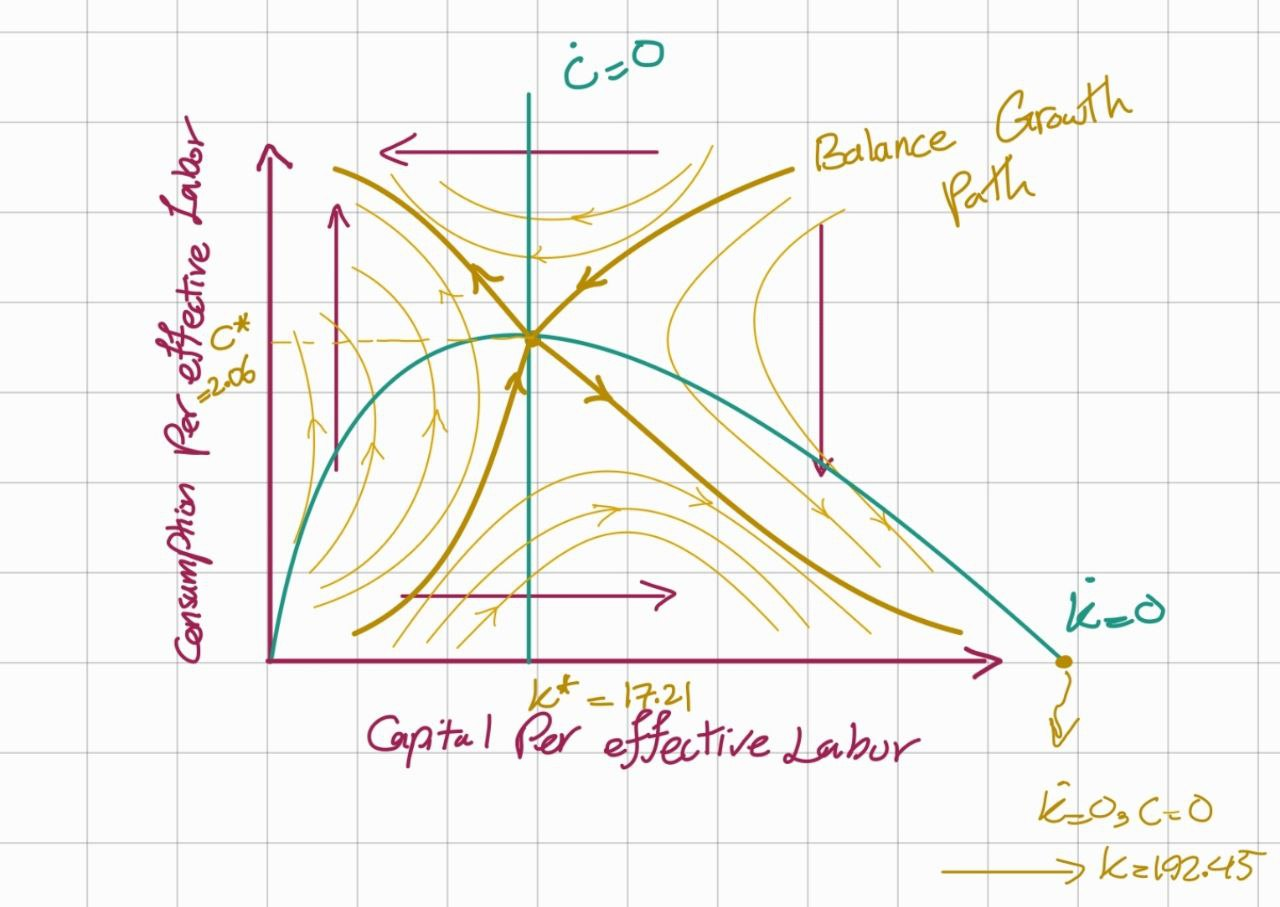
\includegraphics[width=16cm]{3-3.jpg}
\end{figure*}
\newpage
%%%%%%%%%%%%%%%%%%%%%%%%%%%%%%%%%%%%%%%%
%%%%%%%%%%%%%%%%%%%%%%%%%%%%%%%%%%%%%%%%
\problem{4.} Drive the adjustment rate for this dynamic system using the first order Taylor approximation to this
non-linear two-state dynamic system and show that the only stable solution is\\
$$\mu_1=\dfrac{1}{2}\left(\beta-\left[\beta^2+\dfrac{4}{\theta}\dfrac{1-\alpha}{\alpha}(\rho+\theta g)\left[\rho+\theta g - \alpha(n+g)\right]\right]\right)$$\\
Then use this equation to graph $\mu_1$ as a function of $\theta$ and $\alpha$.\\
\begin{center}
    \large\textbf{To open the python code for this problem: \href{run:3-4.ipynb}{Click Here}}\\
\end{center}
\begin{figure*}[h!]
    \centering
    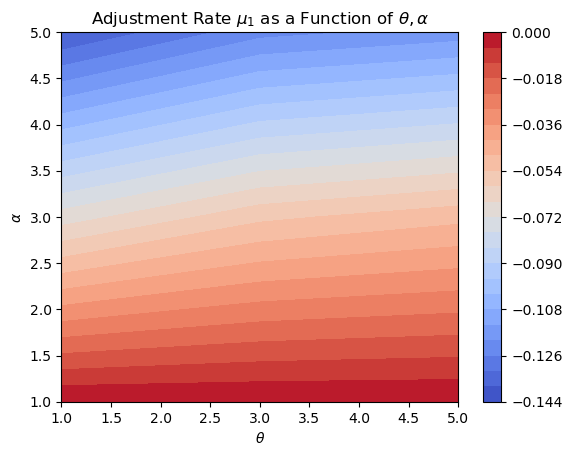
\includegraphics[width=18cm]{3-4.png}
\end{figure*}


\newpage
%%%%%%%%%%%%%%%%%%%%%%%%%%%%%%%%%%%%%%%%
%%%%%%%%%%%%%%%%%%%%%%%%%%%%%%%%%%%%%%%%
\problem{5.} Write a Julia or a Python code to simulate this phase diagram.\\\\
\begin{center}
    \large\textbf{To open the python code for this problem: \href{run:3-5.ipynb}{Click Here}}\\
\end{center}
\begin{figure*}[h!]
    \centering
    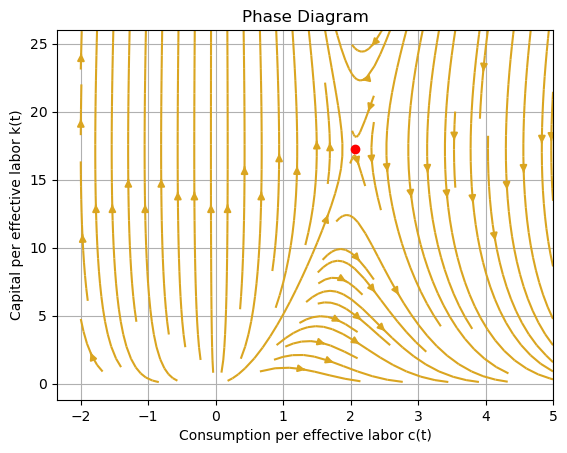
\includegraphics[width=16cm]{3-5.png}
\end{figure*}
\newpage
%%%%%%%%%%%%%%%%%%%%%%%%%%%%%%%%%%%%%%%%
%%%%%%%%%%%%%%%%%%%%%%%%%%%%%%%%%%%%%%%%
%%%%%%%%%%%%%%%%%%%%%%%%%%%%%%%%%%%%%%%%
\textbf{\large\begin{center}
    {Comparative Statics Analysis of the Speed of Convergence}
\end{center}}
Use the phase diagram and the stable saddle path you derived in the previous section to simulate two economies
that start from $k(0) = k^*/2$ and $k(0) = 1.5k^*$.
%%%%%%%%%%%%%%%%%%%%%%%%%%%%%%%%%%%%%%%%
\problem{1.} Depict the path for consumption, capital, and saving rate over time.\\\\
\begin{figure*}[h!]
    \centering
    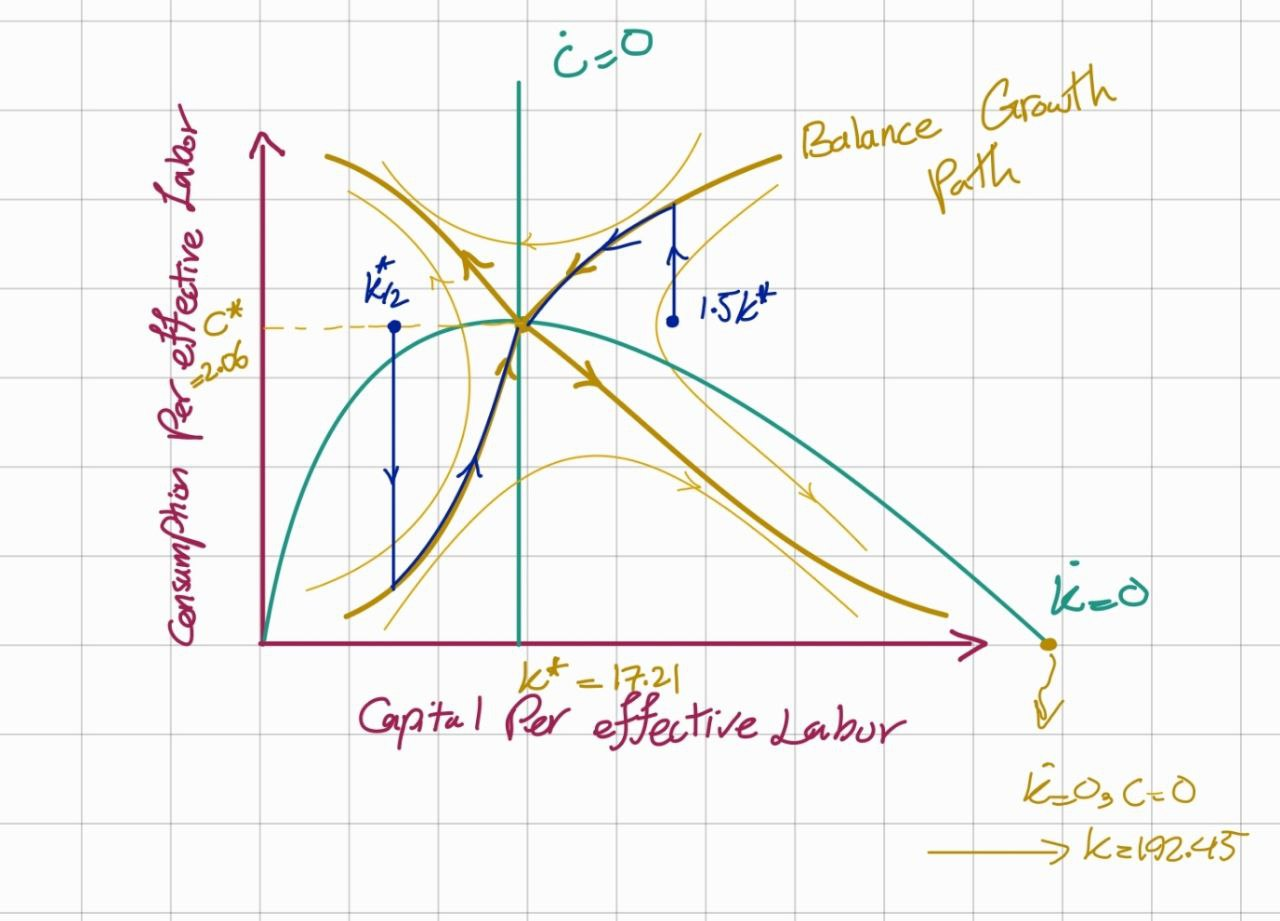
\includegraphics[width=12cm]{4-1.jpg}
\end{figure*}\\
\begin{figure*}[h!]
    \centering
    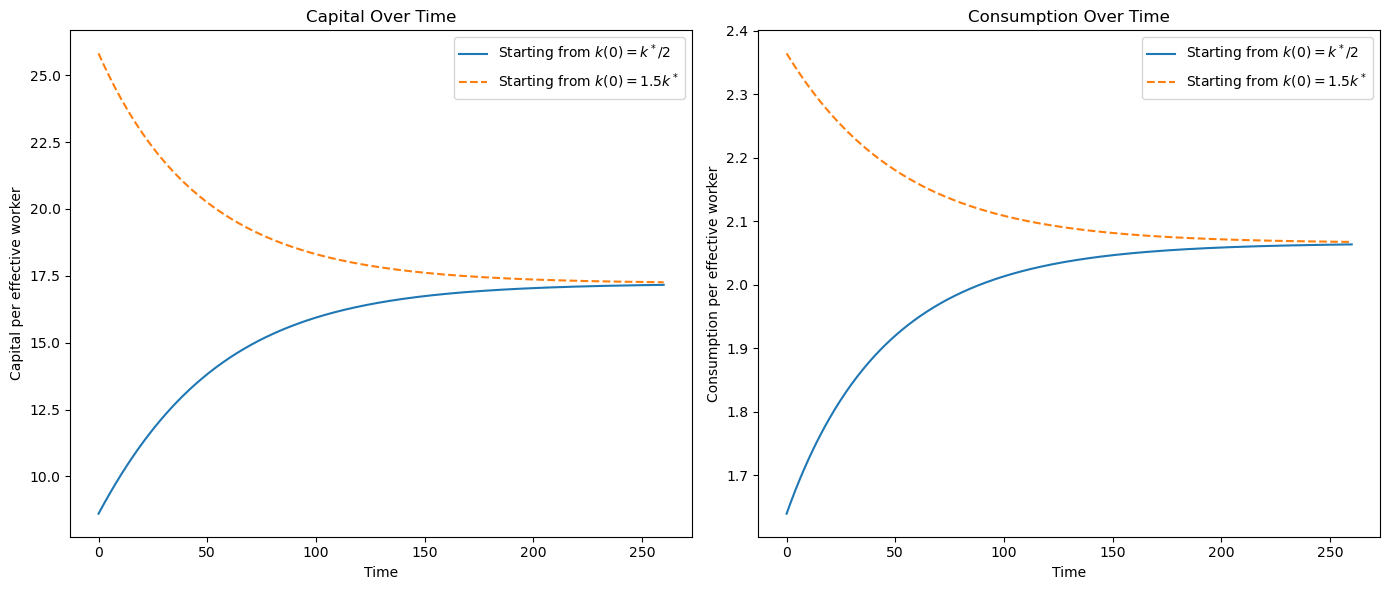
\includegraphics[width=16cm]{4-1-2.png}
\end{figure*}
\newpage
%%%%%%%%%%%%%%%%%%%%%%%%%%%%%%%%%%%%%%%%
%%%%%%%%%%%%%%%%%%%%%%%%%%%%%%%%%%%%%%%%
\problem{2.}Now suppose that $\theta=4$. How would the steady state change? Depict the time path for the above
economies and compare the speed of convergence.\\\\
\begin{align*}
    4\times(\dfrac{1}{3}k^{-2/3}-0.04-0.04)&=0\\
    \implies k^*&=8.51\tag{$\star$}\\\\
    k^{1/3}-c-(0.01+0.02)k&=0\\
    \implies c&=\sqrt[3]{k}-0.03 k\tag{$\star \star$}
\end{align*}\\
Substituting $(\star)$ into $(\star \star)$, we get: $$c^*=1.79$$\\
A higher $\theta$ implies greater risk aversion,
meaning that consumers prefer a smoother consumption path over time (Low intertemporal Elasticity).
So when receiving a shock, the household prefers to smooth the shock over the periods and the rate of convergence would be lower.
(The graphs in part 3-4 also confirms that with increase of $\theta$, rate of convergence decreases.)

\newpage
%%%%%%%%%%%%%%%%%%%%%%%%%%%%%%%%%%%%%%%%
%%%%%%%%%%%%%%%%%%%%%%%%%%%%%%%%%%%%%%%%
\problem{3.} How would the steady state depend on the parameters of the model? Use graphical analysis to justify
your answer and explain the intuition for this result.\\\\
\textbf{Time Preference Rate (\( \rho \))}

This affects how much households value current consumption over future consumption.
A higher \( \rho \) leads to a lower steady state of capital and consumption because households prefer consuming today rather than saving for the future.\\\\
\textbf{Rate of Technological Progress (\( g \))}

Technological progress increases the efficiency of both capital and labor.
In the RCK model, a higher \( g \) leads to a higher steady state of consumption but may have ambiguous effects on the steady state of capital due to its impact on the marginal productivity of capital.\\\\
\textbf{Population Growth Rate (\( n \))}

A higher population growth rate requires more investment to maintain the capital per effective worker ratio,
leading to a lower steady state level of capital per effective worker.\\\\
\textbf{Capital's Share of Output (\( \alpha \))}

This determines the distribution of income between capital and labor.
A higher \( \alpha \) means capital has a higher share, leading to a higher steady state level of capital and output.\\\\
\textbf{Elasticity of Intertemporal Substitution (\( 1/\theta \))}

This parameter influences how willing households are to substitute consumption over time.
A higher $\theta$ (means lower elasticity) implies that households prefer a smoother consumption! 
\newpage
%%%%%%%%%%%%%%%%%%%%%%%%%%%%%%%%%%%%%%%
%%%%%%%%%%%%%%%%%%%%%%%%%%%%%%%%%%%%%%%%
\problem{4.} How would the speed of convergence toward the steady state depend on the parameters of the model?
Use graphical analysis to justify your answer and explain the intuition for this result. You may use
half-life analysis for this part.\\\\
\textbf{Time Preference Rate (\( \rho \))}

A higher \( \rho \) leads to a slower convergence, because households are willing more to current consumption than future consumption,
leading to less saving and investment.\\\\
\textbf{Rate of Technological Progress (\( g \))}

An increase in \( g \) can lead to faster convergence by increasing the productivity of capital and labor. Although if $g$ is too high (in the wonder land!),
we might not be able to catch up and get back on the balance growth path.\\\\
\textbf{Population Growth Rate (\( n \))}

A higher \( n \) increases the effective depreciation rate of capital due to the need for more investment to maintain the capital per effective worker ratio,
probably slowing convergence.
\textbf{Capital's Share of Output (\( \alpha \))}

A higher \( \alpha \) increases the marginal product of capital,
which speeds up convergence.\\\\
\textbf{Elasticity of Intertemporal Substitution (\( 1/\theta \))}

A lower elasticity (higher \( \theta \)) implies that households are less willing to shift consumption over time,
slowing the speed of convergence.\\\\
%%%%%%%%%%%%%%%%%%%%%%%%%%%%%%%%%%%%%%%%
%%%%%%%%%%%%%%%%%%%%%%%%%%%%%%%%%%%%%%%%
%%%%%%%%%%%%%%%%%%%%%%%%%%%%%%%%%%%%%%%%
\end{document}




Substituting the Taylor approximation into the Euler equation gives:
$$ \frac{u'(c_t)}{u'(c_t) + u''(c_t) \cdot \Delta c} = \beta (F'(k_{t+1}) + 1 - \delta) $$\\
Solving for \(\Delta c\) gives the dynamics of consumption:
$$ \Delta c = \frac{u'(c_t) - \beta (F'(k_{t+1}) + 1 - \delta) \cdot u'(c_t)}{u''(c_t) \cdot \beta (F'(k_{t+1}) + 1 - \delta)} $$\\

The first-order Taylor approximation of \(u'(c_{t+1})\) around \(c_t\) is:
$$ u'(c_{t+1}) \approx u'(c_t) + u''(c_t) \cdot \Delta c $$
From the dynamics of capital and consumption, we can find the steady state conditions,
Setting these equal to zero gives:\\
\begin{align*}
    \Delta k &= i_t - \delta k_t = 0 \\
    \implies k^*&=\dfrac{i_t}{\delta}\\
\end{align*}
\begin{align*}
    \Delta c &= \frac{u'(c_t) - \beta (F'(k_{t+1}) + 1 - \delta) \cdot u'(c_t)}{u''(c_t) \cdot \beta (F'(k_{t+1}) + 1 - \delta)} = 0
\end{align*}\\
The following information are also given:
$$F'(.)>0,\;\;F''(.)<0,\;\;\;U'_t>0,\;\;U''(t)>0$$
%%%%%%%%%%%%%%%%%%%%%%%%%%%%%%%%%%%%%%%%

This is the Euler equation for the neoclassical growth model. It represents the intertemporal optimality condition for consumption. The left-hand side is the marginal rate of substitution between consumption in two periods, and the right-hand side is the marginal rate of transformation. In equilibrium, these two must be equal.



Alternatively, we can use Taylor approximation to approximate the dynamic of consumption:
The first-order Taylor approximation of \(u'(c_{t+1})\) around \(c_t\) is:
$$ u'(c_{t+s+1}) \approx u'(c_{t+s}) + u''(c_{t+s}) \cdot \Delta c $$
$$\Delta c \approx -\rho \dfrac{(c_{t+s+1}^{-1/\rho} - c_{t+s}^{-1/\rho})}{c_{t+s+1}^{-1/\rho\;-1}}$$


